\graphicspath{ {imgs/} }
\documentclass[main.tex]{subfiles}
\begin{document}
\chapter{Bandit A/B Testing}
\section{Underlying Idea}
The previous chapter dealt with optimizations concerning classical A/B Testing. The following will describe a fundamentally different approach. Classical A/B Testing focuses solely on gaining information about the different buckets, enabling teams to implement the best performing solution. In the bandit setting this separation between the exploration and the exploitation phase is abrogated. This is motivated by the idea that valuable costumers can be lost during exploration. Basically this means that we want to already maximize our profit while gaining information about the different buckets. When combining exploration and exploitation one has to choose on each step if a known good bucket should be used again or if one invests in other unknown buckets to gain more information about their individual reward function. This balancing is the core of the now described algorithms.

\subsection{Bandit Algorithms}
Bandit algorithms originate from machine learning where they serve learning agents like autonomous robots to show sensible behavior while exploring the environment. In each time step an agent is forced to make a choice among several actions. An action will lead to a reward. The reward function for any action is unknown and the agent can only estimate the true reward function by learning from the generated outcomes. The objective for any agent is to maximize the received reward over the whole experiment. The name of this class of algorithms stems from their relation to the famous casino slot machines called one-armed bandits. Each action can be imagined as the pull of one lever in a row of many of those machines. Each bandit has a hidden reward function and a player wants to maximize her earned money over the course of the evening. The rule for updating the estimate about each machines reward function can be roughly formalized as:
\begin{align*}
NewEstimate \leftarrow OldEstimate + StepSize[Reward - OldEstimate]
\end{align*}
Where the $OldEstimate$ is what the player assumed about the reward that is generated by playing this machine. $Reward$ is the value the payer observed after choosing the action and the $StepSize$ is a value that modulates the learning rate. Based on those information a new estimate is formed about the machine. A K-armed bandit problem is defined by random variables $X_{i,n}$ for $1 \leq i \leq K$ and $n\geq1$ where each $i$ is the index of a slot machine and $n$ the number of times a specific machine has been played. Successive plays of machine i yield reward $X_{i,1},X_{i,2},...$ which are independent and identically distributed according to an unknown reward distribution with unknown expectation $\mu_i$. The machines among themselves are also independent.

\subsection{Reformulating A/B Testing}
Each new user is the chance to either explore or exploit what is known about the buckets of the test. Each assignment becomes the pull on a lever. Since the setup is ignorant towards returning users, the assignments are independent and identically distributed. The A/B Test describes a stationary environment which means our $StepSize$ is $\frac{1}{k}$ where $k$ denotes the total number of assignments for one test. No prior knowledge is assumed before running the test. This translates to no data or knowledge that is not deducible from the single trials, in machine learning such information is called \emph{side information}. The reward value does not differ among the different levers. It is always $1$, although it could be in fact another fixed value. One of the later described algorithms~\ref{ssc:ucb} does require the reward of a lever to be bounded by 1, but for the sake of A/B Testing the concrete value does not matter and can be adapted as seen fit -- it only has to be greater than $0$ and the same for each bucket. What differs though are the real distributions underlying the variations represented by the buckets. These are of the form $P_B(y|w)$ where $w$ are the unknown parameters that define the distributions function. By assigning users we generate random observations $D_B=(y_1,y_2..y_t)$. These observations are used to estimate the difference between the buckets. The test ends after a given number of assignments -- this number is called the \emph{horizon}.

\section{Bandit algorithms}
\subsection{epsilon-greedy}
One of the simplest algorithms exploits always the best performing bucket (with the highest conversion rate) except for $\epsilon $'s fraction of cases where the next bucket is chosen randomly. For example if $\epsilon = 0.1$ then every tenth assignment would not necessarily be to the so far best performing bucket. This means that even after convergence for the bucket probabilities $10\%$ of the assignments will not always hit the optimal bucket. This can be formulated for $n$ buckets as follows:
\begin{align*}
P(exploration) \cdot P(\neg best bucket | exploration) = \epsilon \cdot \frac{n-1}{n}
\end{align*}
A simulation of $1000$ tests, with two random buckets and a horizon of $1000$ and varying $\epsilon$ result in Figure~\ref{fig:EpsGreedy} for the performance of this algorithm. Note that this algorithm does not track or account for the uncertainty of the estimates it has about the buckets. And since it has no `sense' of time (the algorithm does not change if the experiment is almost over and only $m \ll n$ choices left) the epsilon-greedy performs equally well if the environment changes and users behavior change later on.

\begin{figure}[ht]
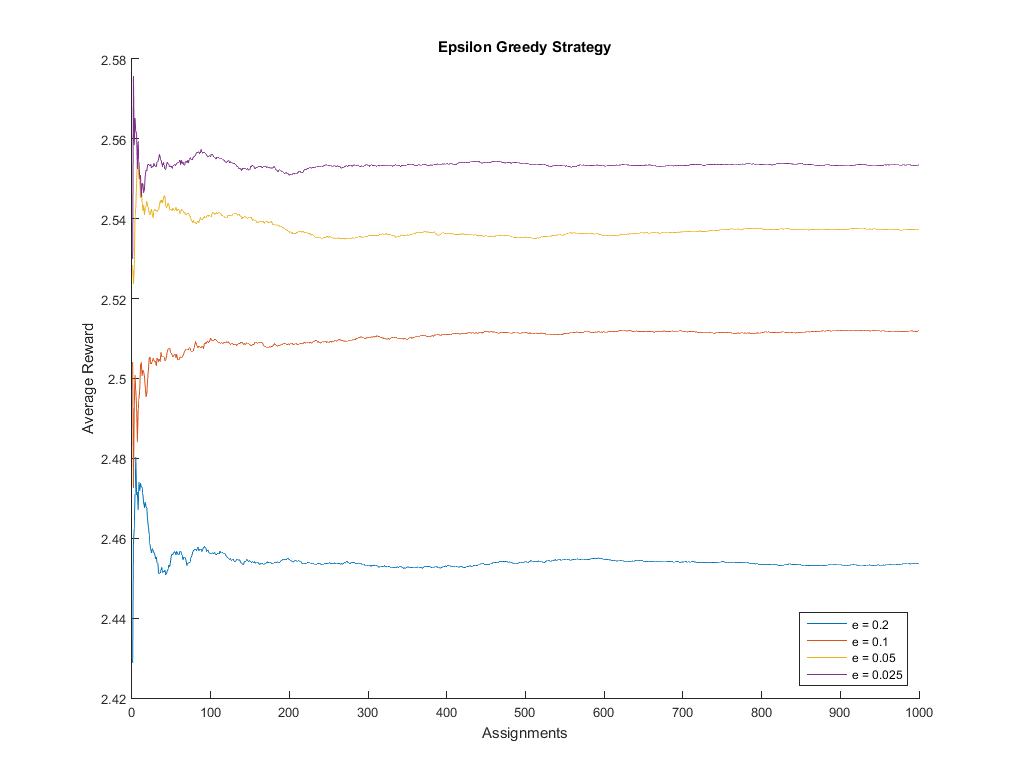
\includegraphics[scale=0.6]{epsGreedy.png}
\centering
\caption{Epsilon Greedy}
\label{fig:EpsGreedy}
\end{figure}
\begin{figure}[ht]
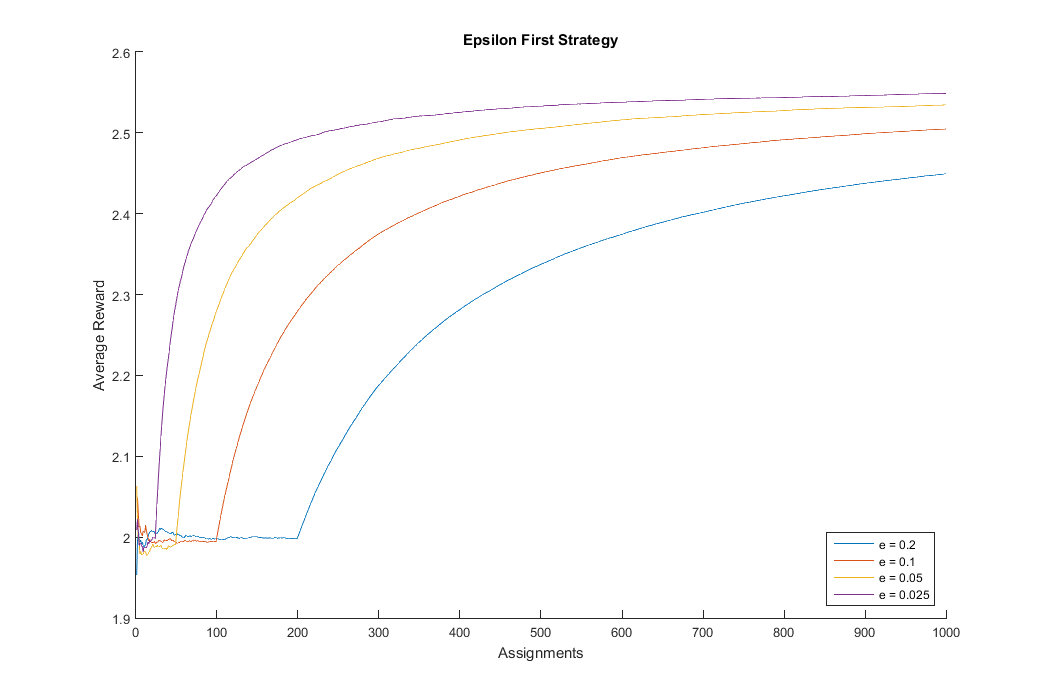
\includegraphics[scale=0.6]{epsFirst.png}
\centering
\caption{Epsilon First}
\label{fig:epsFir}
\end{figure}
\clearpage

\subsection{epsilon-first}
Another algorithm that is closely related is called the $\epsilon$-first algorithm. This is close to A/B Testing since the exploration phase proceeds the exploitation phase for a finite number of steps and afterwards just exploits. This resembles the case where the tested change with the highest payoff is implemented and from then on permanently presented to all users, see Figure~\ref{fig:epsFir}. Since the assigned bucket is fixed after $\epsilon \cdot n$ steps this algorithm can not react to changes that later on happen in the environment.

\subsection{Unified Confidence Bound}\label{ssc:ucb}
The concrete formulas in this section are taken from ``Finite-time analysis of the multiarmed bandit problem'' by Auer~et~al.\,~\cite{auer2002finite}, but the algorithm itself is known across the community. UCB (which stands for \emph{Uniform Confidence Bound}) does not explore for a fixed number of assignments, but dynamically changes the chances for not so good performing buckets to be chosen. The Hoeffding's inequality gives a confidence bound that models how sure we are about the estimated payoff across multiple plays. This way -- the longer we do not play a machine the more likely it will be played in the future (but only once). We choose to play the next machine that maximizes:
\begin{align*}
mean(b_n) + \sqrt{\frac{2\log{N}}{n_p(b_n)}}
\end{align*}
Here $b_n$ is one of $n$ buckets and $n_p(b_n)$ is the number of times this bucket has been played. $N$ corresponds to the number of assignments across all buckets. This algorithm requires $mean(b_n)$ to be bounded by 1 so that the confidence bound overpowers the first term. This is given by our assumption that the concrete value of the individual rewards does not matter as long as they are the same across buckets. The fraction of time that is spend on exploring decreases exponentially.


\subsection{Thompson sampling}\label{ssc:thompson}
This fairly simple algorithm was originally developed by William R. Thompson in his paper ``On the likelihood that one unknown probability exceeds another in view of the evidence of two samples''~\cite{thompson1933likelihood}. To determine the next bucket to be played, the buckets probability distribution itself is used. The result of that sampling is used to update the buckets underlying distribution as described in \ref{sec:setup}.

\begin{algorithm}
\SetKwData{nb}{nextBucket}\SetKwData{nbs}{nextBucketSuccess}\SetKwData{i}{i}\SetKwData{r}{rew}
\SetKwData{nbf}{nextBucketFailures}
\SetKwArray{b}{buckets}\SetKwArray{d}{draws}
\SetKwFunction{max}{maxarg}\SetKwFunction{draw}{draw}\SetKwFunction{rw}{reward}
\SetKwFunction{updFail}{updateBucketFailure}\SetKwFunction{updSuc}{updateBucketSuccess}
\KwIn{\b}
%\KwOut{\na}
\BlankLine
\d $\leftarrow$ zeroes \;
\ForEach{\i in \b }
{
\d(\i) $\leftarrow$ \draw{\b{\i}}
}
\nb $\leftarrow$ \max{\d} \;
\r = \rw{\nb}\;
\eIf{\r == 1}{
\updSuc{\nb};
}{
\updFail{\nb};
}

\caption[Thompson sampling]{The usage of Thompson sampling}
\label{alg:ThompsonSampling}
\end{algorithm}

They generate numbers that naturally balance between exploitation and exploration, because less performing buckets are demoted and winners promoted by the information already collected. This method is as well resistant to changes in the environment since they `notice' the change by playing a less performing bucket, that will then be played more often if its performance increased. A comparison between Thompson Sampling and the UCB-Algortihm described in \ref{ssc:ucb} can be found in \ref{fig:ThompsonVsUCB}. Here the UCB is weaker in the first part of assignments but slightly outperforms the Thompson sampling in the long run. A paper that is taking a look at the general performance of Thompson sampling versus UCB for more arms is ``An empirical evaluation of Thompson sampling'' by Chapelle and Li~\cite{chapelle2011empirical}. They show that in the general case Thompson sampling outperforms UCB.

\begin{figure}[ht]
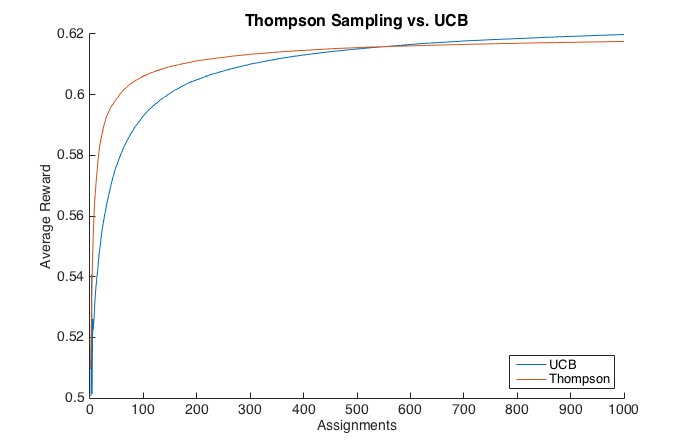
\includegraphics[scale=0.6]{ThompsonVsUCB.png}
\centering
\caption{Comparison for Thompson sampling and UCB}
The graph averages $1000$ runs with random bucket distributions and a horizon of 1000.
\label{fig:ThompsonVsUCB}
\end{figure}

\subsection{Discussion}
The section started with a weaker Bandit algorithm: epsilon-greedy. The major drawback on that was the fact that the exploration phase did not adapt to the gained insights of the different buckets. But still: for this simplified scenario it works well compared to the other algorithms. This is due to two major restrictions that were imposed on the problem. First only two buckets were used in the A/B Test, for more buckets the performance of epsilon-greedy would reduce since the number of not optimal played buckets $\epsilon \cdot \frac{n-1}{n}$ grows for increasing number $n$ of buckets. Another assumption was that the reward functions of the buckets do not change throughout the test. This is especially important for epsilon-first since this method is not sensitive to changes that occur after the initial exploration phase.

UCB and Thompson Sampling are stronger algorithms in the way, that they account for changes in the users behavior and their exploration phase is dynamically bound to the information that are collected during the test. This is not taken advantage of in the explored A/B Testing scenario of this thesis since the reward functions do not change with the trials, but can be powerful in any real application.

Bandit algorithms are very useful when they keep on running for an unspecified time. In fact, since most of them distribute new users in a way that over the time most of them experience the `better' variant, they replace the deployment cycle for new features by rolling them out slowly to the customer base.

\end{document}